\documentclass{article}
\usepackage{tikz}
\usetikzlibrary{arrows.meta, positioning}

\begin{document}

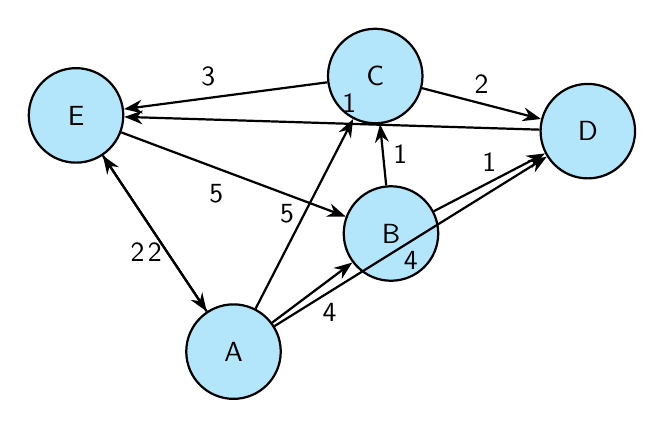
\begin{tikzpicture}[->, >=Stealth, thick,
    node/.style={circle, draw=black, fill=cyan!30, minimum size=1.2cm, inner sep=0pt},
    font=\sffamily
  ]

  % Nodes manually positioned
  \node[node] (A) at (0,0) {A};
  \node[node] (B) at (2,1.5) {B};
  \node[node] (C) at (1.8,3.5) {C};
  \node[node] (D) at (4.5,2.8) {D};
  \node[node] (E) at (-2,3) {E};

  % Edges with weights
  \draw (A) -- (B) node[midway, below right] {4};
  \draw (A) -- (C) node[midway, left] {5};
  \draw (A) -- (D) node[midway, below] {4};
  \draw (A) -- (E) node[midway, below left] {2};

  \draw (B) -- (C) node[midway, right] {1};
  \draw (B) -- (D) node[midway, above] {1};

  \draw (C) -- (D) node[midway, above] {2};
  \draw (C) -- (E) node[midway, above left] {3};

  \draw (D) -- (E) node[midway, above right] {1};

  \draw (E) -- (A) node[midway, below] {2};
  \draw (E) -- (B) node[midway, below left] {5};

\end{tikzpicture}

\end{document}